%\documentclass[conference,compsoc,a4paper]{IEEEtran}
\documentclass[10pt,conference]{IEEEtran}

\usepackage{array}
\usepackage[utf8]{inputenc}   % <<<<< Linux
\usepackage[nomain,acronym,xindy,toc]{glossaries} 
\usepackage{tabularx} 
\usepackage{float}

\usepackage{cite}    
\usepackage{graphicx,flafter}
\graphicspath{{../tese2/} {.}}

\usepackage{color, colortbl}
\definecolor{Gray}{gray}{0.9}

\usepackage{url} 



\hyphenation{op-tical net-works semi-conduc-tor}
\loadglsentries[main]{xacronyms}

\newcolumntype{Y}{>{\centering\arraybackslash}X}
\newcolumntype{M}[1]{>{\centering\arraybackslash}m{\linewidth/#1}}

\begin{document}


\title{Hyper-linked Communications: WebRTC enabled asynchronous collaboration}

\author{\IEEEauthorblockN{Henrique Rocha}
\IEEEauthorblockA{INESC-ID / Instituto Superior T\'{e}cnico\\
Av. Prof. Dr. Anibal Cavaco Silva\\
2744-016 Porto Salvo, Portugal\\
Email: henrique.rocha@tecnico.ulisboa.pt}
\and
\IEEEauthorblockN{Ricardo Lopes Pereira}
\IEEEauthorblockA{INESC-ID / Instituto Superior T\'ecnico \\
Av. Prof. Dr. Cavaco Silva\\
2744-016 Porto Salvo, Portugal\\
Email: ricardo.pereira@inesc-id.pt}
}

\maketitle

\begin{abstract}
The Hyper-linked communications concept applies much of the hypermedia concepts, widely used on Web content, to the communications realm.
This paradigm allows to synchronize, structure and navigate communication content integrated into voice and video calls.
Voice and image together can express emotions like no other medium can. 
With hypermedia concepts, we can add even more value to conference calls.

This paper describes the design, implementation and evaluation of a hyper-media communication platform targeting the web platform and making use of \emph{WebRTC} technology.
Our prototype provides a hyper-linked, non-linear, multi-party video conferencing platform with support for multiple media types, collaborative text editor, time annotations, instant messaging and a mechanism to superimpose hyper-media to video.

%Our prototype was built using a hybrid peer-to-peer and client-server architecture, resorting to open source software.
Usability tests using 20 users evaluated our prototype positively: 100\% considered it innovative and 95\% recommended its use. 
From a deployment point of view, our performance tests showed that our solution was expensive to scale up, even though the cost could be significantly lowered by disabling some of the advanced functionality.


\end{abstract}

\IEEEpeerreviewmaketitle

\section{Introduction}
\label{chapter:introduction}


As communications technologies evolved, we adapted the way we communicate. 
Multi-party video conference is today a commonly used tool in the enterprise, academia and individually.
The \gls{WWW} has made us familiar with the concept of text hyper-media, in the form of hyper-links.
\gls{IPTV} and video hosting platforms, such as Youtube, made non-linear video watching a common practice.
The latter also use the concept of hyper-links superimposed over videos.
However, these three concepts, video-conferencing (which is real-time), non-linear video watching and hyper-media, have largely remained independent concepts.

This paper describes our efforts to develop a prototype that combines these three concepts, providing a video-conferencing web application that allows users to navigate back and forth in time to catch up on what was said, while the video-conferencing is going on.
We developed a collaboration application, targeted at the web platform resorting to \gls{WebRTC}, that leverages the hyper-linked communications concept by providing a video conference environment enriched with interactive and non-interactive discrete media types such as images, subtitles, forms and all types of content that can be added using \gls{HTML}5, \gls{CSS}3 and \emph{JavaScript}.
Our collaboration application also includes a collaborative text editor and a chat that supports sending time hyper-links and files to conference participants.

One of the key features of this project is the ability to navigate in time in order to reproduce the conversation again.
Users can use a time bar to navigate in time: rewinding communications, fast-forward or jump to a certain point in time.
Time hyper-links also enable accessing the collaboration (video, chat, text editor, etc) at a given instance in time.
Users are capable of enriching the video content, in real-time or at a latter time, by adding content to it, such as timed annotations, interactive lists of topics and subtitles, thus also improving content search abilities.
In this context, we also provide a method for real-time creation and synchronizing of hyper-linked content using \gls{QR} codes.

We envision the use of our collaboration platform in many situations, such as: virtual classroom, where students can interact with the professor during class and later review the subjects, while the latter can enrich the recording with extra materials and annotation after the lecture; recording meetings, where the video stream can be annotated and bookmarked with the agenda points, and support documents added.

The remainder of this paper is organized as follows.
Section \ref{chapter:relatedwork} provides a background on the field.
Section \ref{chapter:architecture} describes the requirements we defined for our system and architecture for fulfilling them.
The choices performed for the implementation of our prototype are presented in Section \ref{chapter:implementation}.
In Section \ref{chapter:evaluation} we present the evaluation tests performed and their results.
Section \ref{chapter:conclusion} summarizes the work developed and proposes future work.









\section{Background}
\label{chapter:relatedwork}


\emph{Hypertext} is a type of text that provides links to texts or other types of content, these links are known by \emph{hyperlinks}. 
\emph{Hypermedia} is an evolution of \emph{hypertext}, it includes audio, images, text and video. 
\emph{Hypermedia} concept brings the possibility to organize and overlay multimedia elements into a nonlinear structure~\cite{geddes}.

Some \gls{MPEG} implementations added hypermedia information to empty space present on \gls{MPEG} frames in order to provide interactive television, modifying the \gls{MPEG} encoder and decoder in order to handle hypermedia content~\cite{embedded}.

Hyper-video is a kind of video that contains links to any kind of hypermedia, including links to skip part of it. An example of hypermedia application could be a search engine over hypermedia content, like subtitles, in order to jump to a specific time in a video or audio track.
\emph{HyperCafe} was an experimental project to expose hyper-video concepts that consisted of an interactive film that enabled switching between different conversations taking place inside a cafe~\cite{hypercafe}.
 
Detail-on-demand is a subset of hyper-video that allow us to obtain additional information about something that appears along the video, like obtaining information about a painting that appears in a particular segment. 
\emph{Hyper-Hitchcock} is an editor and player of detail-on-demand video~\cite{hitchcock}.

\emph{HyVAL}~\cite{hyval} is an \gls{XML} based language that was proposed for modeling composition, synchronization and interaction of hypermedia. 
HyVAL defines defines video structure, internal video and external media objects. 
\emph{HyVAL} uses a primary video stream, around which all other elements are organized and synchronized.
\emph{HyVAL}'s video structure object defines a structure derived from traditional video, which divides video into segments, scenes, shots and frames hierarchically. 
  This approach is quite restrictive if we want to apply hyper-video concepts to videos that do not follow this structure. 
%External media objects are linked by primary video, those objects can represent other videos, images, text, animation and sound.
  %RP não percebo bem a última frase. O que é primary video?

  \gls{SMIL}~\cite{smil} was introduced to describe temporal behavior of multimedia content%, in particular, it could be used to overlay subtitles on films%
  . 
With \gls{SMIL} it is possible to synchronize multiple videos, either in parallel or in sequence, reproduce a different audio track, overlay user interface elements like subtitles or hyper-links, among multiple other features.
  %RP synchronize multiple sections of video? vários videos apresentados em simultâneo?

 % \gls{SMIL} is an \gls{XML} based language that defines twelve modules: \emph{Animation}, \emph{Content Control}, \emph{Layout}, \emph{Linking}, \emph{Media Objects}, \emph{SmilText}, \emph{Meta Information}, \emph{Structure}, \emph{Timing}, \emph{Time Manipulations}, \emph{State} and \emph{Transitions}.


%The \gls{DOM} is a standard \gls{API} that allows easy management of documents that are organized in a tree structure, by providing \gls{CRUD} operations over its elements and their attributes. \gls{DOM} makes it easy to inter-operate between imperative and declarative programming languages~\cite{dom}.
%RP não arranjas uma referência para o dom?

%Like \gls{DOM}, \gls{SMIL} \gls{DOM} is an \gls{API} for \gls{SMIL} documents. Allowing \gls{CRUD} operations over \gls{SMIL} documents is an important feature for extending \gls{SMIL} capabilities, for example for creating non-linear animations and triggering external events like \emph{JavaScript} functions.  
  
%  \gls{SMIL} fits our goals for creating a multimedia rich hyper-call, but it lacks on browser compatibility. Ambulant \cite{ambulant} was one of the SMIL players that were developed for browsers, although this player implements most of \gls{SMIL} 3.0 \cite{smil3} specifications, it needs to be installed on browsers as a plug-in.

%  SmillingWeb \cite{smillingweb} attempts to implement a cross platform multimedia player designed for \gls{SMIL} 3.0 presentations with \emph{JavaScript} and \emph{jQuery} which, unlike \cite{ambulant}, does not require a plug-in to be installed and should not have incompatibility issues. 
%  SmillingWeb already takes advantage of \gls{HTML}5 and \gls{CSS}3.
%  It takes into account unsupported web browsers through the use of \emph{Modernizr}\footnote{\url{http://modernizr.com/}(accessed June 2, 2015).}, a simple \emph{JavaScript} library that may require plug-ins if new features are not supported.  
%  But SmillingWeb just implements a subset of \gls{SMIL} 3.0 and their scheduler engine loads the \gls{SMIL} file only once, which could raise problems when dealing with \gls{SMIL} changes due to real time communications.
 % Another problem with SmillingWeb is pre-loading and playing elements at the correct interval of time, which is not always possible due to high latency networks leading to  pauses during playback.

 % An alternative to \gls{SMIL}'s \emph{Layout} module is to use \gls{HTML} which is a markup language based on \gls{XML} that is used for creating web pages. \gls{HTML} alone is a very poor language when we are focused on visual appealing and interactive web pages. Languages like \gls{CSS} and \emph{JavaScript} are typically used along with \gls{HTML} for improving the interaction and appearance of a web page. 






  With the emergence of \gls{HTML}5, tags like \emph{video}, \emph{audio} and \emph{track} allow us to play video with multiple \emph{codecs}, audio and subtitles in \gls{WebVTT} format.
Another important tag is \emph{canvas} that allows drawing graphics with \emph{JavaScript} on a rectangle within a web page.

%  For example, with \gls{API}s like WebGL\footnote{\url{http://khronos.org/webgl/}(accessed June 2, 2015).}, it is now possible to manipulate a three dimensional environment in the context of a hyper-call. Another example would be a collaborative spreadsheet using \gls{WebRTC}. With this, hyper-calls are not limited to only audio, image, text and video, but also interaction with complex graphical user interfaces that changes over time.

  \gls{SVG} is an \gls{XML} based format that incorporates the animation module of \gls{SMIL}. Currently, \gls{SVG} allows adding movement and animating attributes of elements. When embedded on \gls{HTML}5, it allows dynamic changes to inner content in real time through the \gls{DOM} \gls{API}. Besides that, it also allows calling \emph{JavaScript} functions on events such as animation end, mouse over and mouse click.
  


\gls{WebRTC} is an open source technology that defines a collection of standard protocols and \emph{JavaScript} \gls{API}s for web browser based real time communications without installing any additional application or plug-in. 
\gls{WebRTC} uses \gls{SDP} \cite{rfc4566} to define peer connection properties such as types of supported media, \emph{codecs}, protocols used and network information. An \gls{SDP} offer describes to other peers the expected type of communication and its details, such as used transport protocols, codecs, security and other.


%Some operating systems such as \emph{Android}, \emph{iOS}, \emph{Linux}, \emph{OSX} and \emph{Windows} implement native \gls{WebRTC} libraries, extending the usage of \gls{WebRTC} to applications outside the web browser. This native support can help to implement applications that record video and audio streams for further playback.

However, \gls{WebRTC} by itself does not define how users get to know each other nor how information flows between users. 
  Signaling is the process by which applications exchange connection information about peers and servers, their capabilities and meta-data.
  In particular, \gls{WebRTC} does not implement signaling, as different applications may require different protocols and there is no single answer that fits all problems.
  As a consequence, multiple options are available for filling the missing \gls{WebRTC}'s signaling component, which can be performed using \gls{SIP}\cite{rfc3261}, \gls{XMPP}, \emph{WebSockets}, \emph{Socket.io}\footnote{\url{http://socket.io/}(accessed June 1, 2015).}, \gls{SigOfly}\cite{sigofly} or by implementing a custom protocol.

 	











\section{Architecture}
\label{chapter:architecture}

From an user experience point of view, we designed our collaboration application around the concept of group conferences (or conference rooms).
Users can create group conferences and invite other users to participate in these, either by adding the other user or by sharing a \gls{URL} (invitation link).
In order to meet user expectation, a group conference provides functionality similar to those found in established applications such as \emph{Skype} or \emph{Google Hangouts}.
Among other common features, one can view a video composed by all participants or a video of a selected participant.
Each participant may use more than one camera, in order to show different angles or objects, e.g. a white board and himself.
The source of the video can be selected manually or be automatically assigned to the talking participant.
Participating users may choose to view only, share their microphone, camera or screen.

Besides the videos, a group conference includes a chat, collaborative text editor, list of users and document sharing.
The major differentiating feature is a time-line bar, for navigating in time.
While the group conference is taking place, this time bar is continuously progressing as time goes by.
The user is free to slide over to any instant in the past or back to real-time.
Changing the instant of time updates the state of not only the video but also of other collaboration elements. % ("other collaboration elements", nao foi implementado, apenas para conteudo sobreposto...) %

Either in real-time or later, users can create bookmarks, displayed in the time-line, for easier navigation in time.
Users can also superimpose content to video.
This content can be as simple as subtitles or as complex as a \gls{HTML} document or JavaScript code to perform an animation or interaction.
All the content is searchable, allowing for time navigation by content.

From an early stage, we decided to target the browser platform, due to its ubiquity and breadth of devices, from desktops, to tablets and smartphones.
The nature of web browser applications already follows the hypermedia concept, which makes \emph{WebRTC} the ideal technology to apply the hyper-linked communications concepts.
The advent of \gls{WebRTC}, currently available on the major web browsers, makes it possible to develop video conference web applications without plugins.
However, mobile devices have limited resources for handling a large number of simultaneous video stream.

\gls{SFU} is a technique that consists on having a server relaying each stream, as it is, to other users. Leaving the stream selection and composition operations to the user.

In order to limit the processing requirement in the client application (browser), we decided to use a server to combine the audio and video streams from all the participants into a single video and a single audio track. This technique is called \gls{MCU}.
This also helps conserve battery on mobile devices.
Each user listens to the combined audio track and may choose to see a single participant or all of them, in this case using the combined video track. 

We realized that it would be useful to add some content, such as bookmarks, an agenda or links to referenced documents, while participating in a conference.
We also realized it would be difficult for the same person to do it while performing a presentation.
As such we devised a method, where the user displays \gls{QR} codes in order to ease content creation.


Figure~\ref{fig:modules} presents the structure of our system, which was divided into six modules:


\begin{figure}
	\centering
	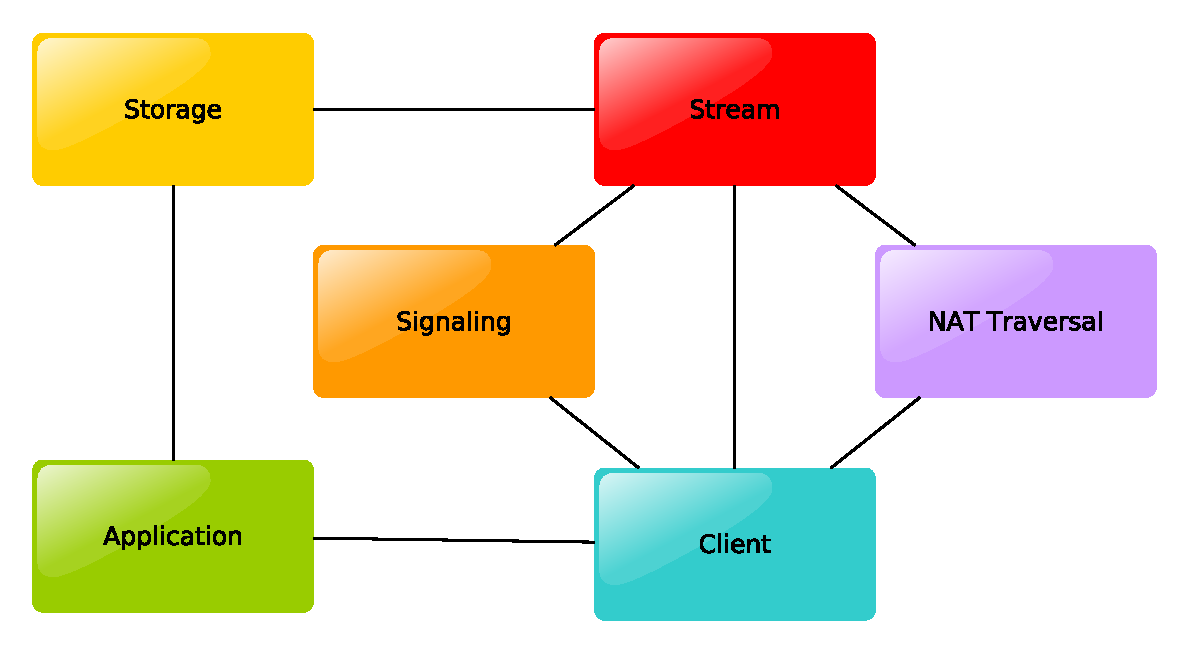
\includegraphics[width=\linewidth]{figures/modules.pdf}
	\caption{System Modules}
    \label{fig:modules}
\end{figure}

\paragraph{Application module} responsible for providing information about the relevant modules (\emph{NAT Traversal} and \emph{Signaling}) and user interface to the \emph{Client} in the form of web pages in \gls{HTML} and \emph{JavaScript} libraries through \gls{HTTP}.
 
\paragraph{Signaling module} responsible for \emph{Client} and \emph{Stream} coordination which will be performed using \emph{WebSockets}.

\paragraph{NAT Traversal module} \gls{STUN} and \gls{TURN} techniques (part of \gls{ICE}) are used by the \emph{Client} and \emph{Stream} modules during the \emph{Signaling} phase that ends with the establishment of the connection between them.

\paragraph{Stream module} responsible to deliver and receive multimedia content from the \emph{Client} using \gls{WebRTC}. This is where audio and video are combined into single streams. It is also here that \gls{QR} codes present in the client streams are detected.

\paragraph{Storage module} provides two main functionalities: store the model information and media recorded. This is the single module responsible for persistent storage. It stores user and communication data as well as all the data required among user sessions. It is used as well to store all the communication streams, so that they can be viewed later.

\paragraph{Client module} responsible for the interaction with the user. It runs on the user device's browser.


Figure \ref{fig:infrastructure} depicts the architecture of our system, being composed by: web server, streaming server (\gls{KMS}), signaling server (\gls{ICE} server), database (MongoDB) and video repository (Kurento Repository).

\begin{figure}
	\centering
	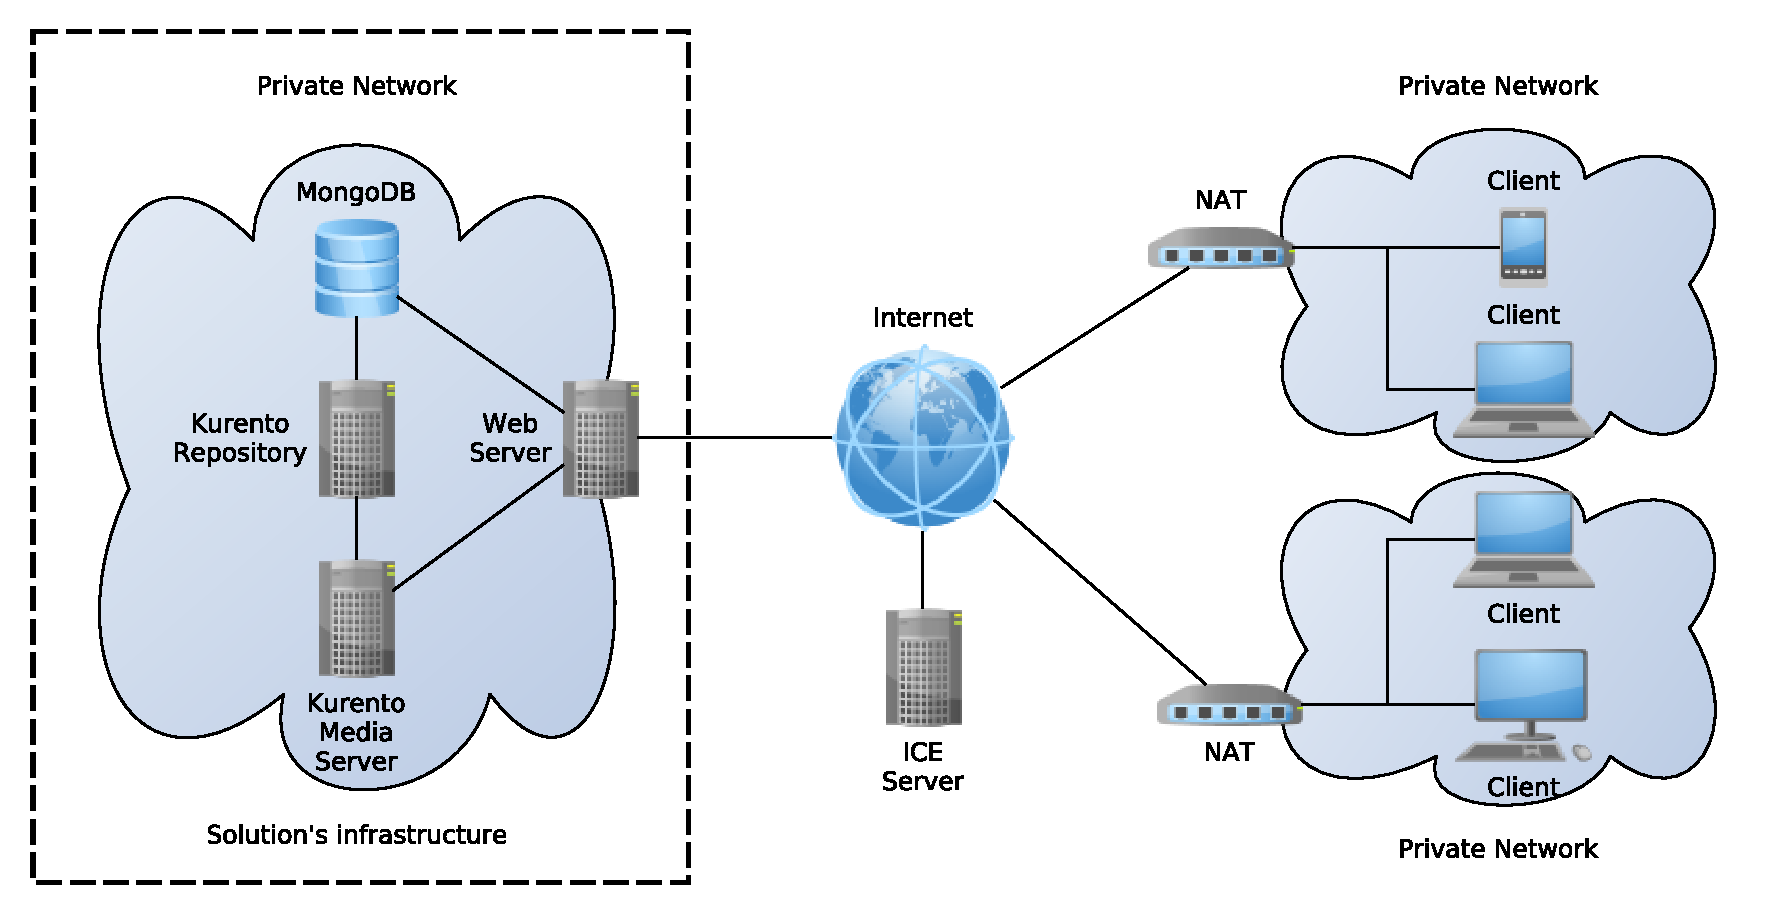
\includegraphics[width=\linewidth]{figures/infrastructure.pdf}
	\caption{System Infrastructure}
        \label{fig:infrastructure}
\end{figure}

In order to simplify our solution, the \emph{Application}, \emph{Signaling}, \emph{Stream} and \emph{Storage} modules are deployed within the same server, as to facilitate deployment.
To this set of modules, we call \emph{backend}.
The \emph{Application} module is split between client and server part.
The \emph{Signaling} module is implemented together with the application server.

(Application) clients can only access the web server, all other servers are in a firewalled private network.
Access to our streaming servers is given to clients after concluding the signaling phase.
This signaling phase may or not proceed in function of the client access permissions to the particular group conference.

With the use of a centralized architecture, each client only has one \emph{PeerConnection} to our streaming server and content shown to them is changed on demand, either being it an individual or a composite view. 
A peer-to-peer approach would have required each peer to maintain a connection to each of the other participants and one to the streaming server, for recording.
This would seriously limit the size of each group conference by placing high bandwidth and processing requirements on the clients. 
The same can be concluded about instant message delivery.
Each client has only one \emph{WebSocket} connection to the application server which consequently relays the messages to other users.

Our architecture can be scaled by having conference rooms distributed across different servers.
However, all of a group conference participants must be connected to the same server.


\section{Implementation}
\label{chapter:implementation}


Our prototype was built using \gls{KMS} as our media streamer, as \gls{KMS} supports \gls{WebRTC}.
The server side of the \emph{Application} and \emph{Signaling} modules are implemented as a server side web application. 
Our server could be implemented with JavaScript (e.g. with \emph{NodeJS}) or \emph{Java} due to the fact \gls{KMS} provides clients for both technologies. 
We decided to implement our web server using the \emph{PlayFramework}\footnote{\url{https://www.playframework.com/}(acessed March 25, 2016)} using \emph{Java}.
For the collaborative text editor, we resorted to \emph{OT.js}\footnote{\url{http://operational-transformation.github.io}(accessed March 10, 2016)} due to its server and storage implementation choice independence.

By default, \emph{Kurento Repository}, used for storing the recorded video and audio streams, is implemented over \emph{MongoDB}.
For convenience, our storage model also uses the same database.
In order to offer all the functionality, some information about objects must be stored on the database, such as users, groups, relations among users, group memberships, messages, hyper-content, recordings and collaborative editor state. 

% persistent -> stored on database, reviewer2 confundiu persistent com fixed 

For the \emph{NAT Traversal} module, a public \gls{STUN} server was used for testing our solution.
Nevertheless, we recognize that for a production environment we would need to maintain our own \gls{TURN} servers in order to ensure connectivity to all clients.




Table~\ref{table:apparch} presents the client application architecture and the underlying technologies used.
Both \emph{Mozilla Firefox} and \emph{Google Chrome} browsers are supported.
\emph{Adapter.js} and \emph{jQuery} ensure that our application is compatible with the most popular web browsers.
\emph{Bootstrap} is used to make the user interface more appellative and responsive, adapting to mobile devices with different screen sizes.
\emph{OT.js} is used to synchronize the collaborative text editor.


\begin{table}
\centering
	\caption{Application Architecture}
	\label{table:apparch}

\resizebox{\columnwidth}{!}{%
    \begin{tabular}{cccccccc@{}m{0pt}@{}}
	\hline 
	\multicolumn{8}{|c|}{\cellcolor{Gray}Application}  &\\[12pt]\cline{1-5}\cline{7-7}
	\multicolumn{1}{|c|}{jQuery} & \multicolumn{1}{c|}{HTML5} & \multicolumn{1}{c|}{CSS3 (Bootstrap)} & \multicolumn{1}{c|}{Signaling} & \multicolumn{1}{c|}{ot.js} & \multicolumn{1}{c|}{\cellcolor{Gray}} & \multicolumn{1}{c|}{adapter.js} & \multicolumn{1}{c|}{\cellcolor{Gray}} &\\[12pt]\hline
	\multicolumn{1}{|c|}{HTTP} & \multicolumn{2}{c|}{User Interface}  & \multicolumn{3}{c|}{WebSocket}    & \multicolumn{2}{c|}{WebRTC}      &\\[12pt]\hline
	\end{tabular}
}
\end{table}

%RP acho interessante o que queres fazer aqui mas acho que está mal conseguido. A linha de baixo, devia ter coisas ao mesmo nível, o que não aconteçe.
% Qual a razão para HTTP estar por baixo do jquery e user interface estar ao lado?
% Sugiro colocar a applicação no meio e as várias interfaces (webrtc, websocket e http) uma de cada lado (esquerda, baixo e direita), indicando o que fica do outro lado (outro cliente, servidor web, servidor stream, etc)


Interaction and synchronization between the streaming server, the application server and the clients is achieved using a signaling protocol.
After the web application server validates the user access, the client creates a WebSocket to exchange signaling information with that server. 
Our signaling protocol consists of sending and receiving \gls{JSON} formated messages over that \emph{WebSockets} by both the application server and the client. 

The Web application server retrieves all the information needed from the database in order to check if the user has permissions to join that conference room. 
It is important to save the user identification before the \emph{WebSocket} connection is created because, after the handshake is performed by the \emph{WebSocket} protocol\cite{rfc6455}, the \gls{HTTP} context is lost.

At this stage, the web application's user is asked if he wants to share its camera and microphone, share screen or just receive streams from the server. 
If the user decides to share his camera or screen the user agent creates an offer, sets a \emph{local session description} to its \emph{PeerConnection} and sends it through the \emph{WebSocket} to the Application Server.
From a \gls{WebRTC} point of view, our media server (\gls{KMS}) is a peer that receives video streams and sends it to its connected peers (the clients). 

Figure \ref{fig:signaling2} shows the sequence of messages, intermediated by the server, by which both client and \gls{KMS} determine and exchange \gls{ICE} candidates for establishing a direct connection despite \gls{NAT} firewalls.

%The server receives and processes the offer and sets the \emph{remote session description} to its client associated \gls{WebRTC} endpoint.
%Then a \emph{local session description} is created on the server and sent back to the client.
%After that, the server tries to gather \gls{ICE} candidates.

%The client receives the server answer, sets the \emph{remote session description} and gets the \gls{ICE} candidates from the \gls{ICE} server.
%Subsequently, both the server and client receive the \gls{ICE} candidates that allow the client to connect directly to \gls{KMS} and vice-versa. 
%The candidates are received at the client which sets them to its \emph{PeerConnection}. 
%The same is done on the server which receives the \gls{ICE} candidates from the client and propagates them to \gls{KMS}.

%An \gls{ICE} candidate contains an \gls{IP}, port, used transport protocol and an attribute named \emph{sdpMLineIndex} that is used for mapping to the \emph{remote session description} media type.
%When a connection is established, the user and server start to interchange stream data but other \gls{ICE} candidates may arrive with better connections.

\begin{figure}
    \centering
    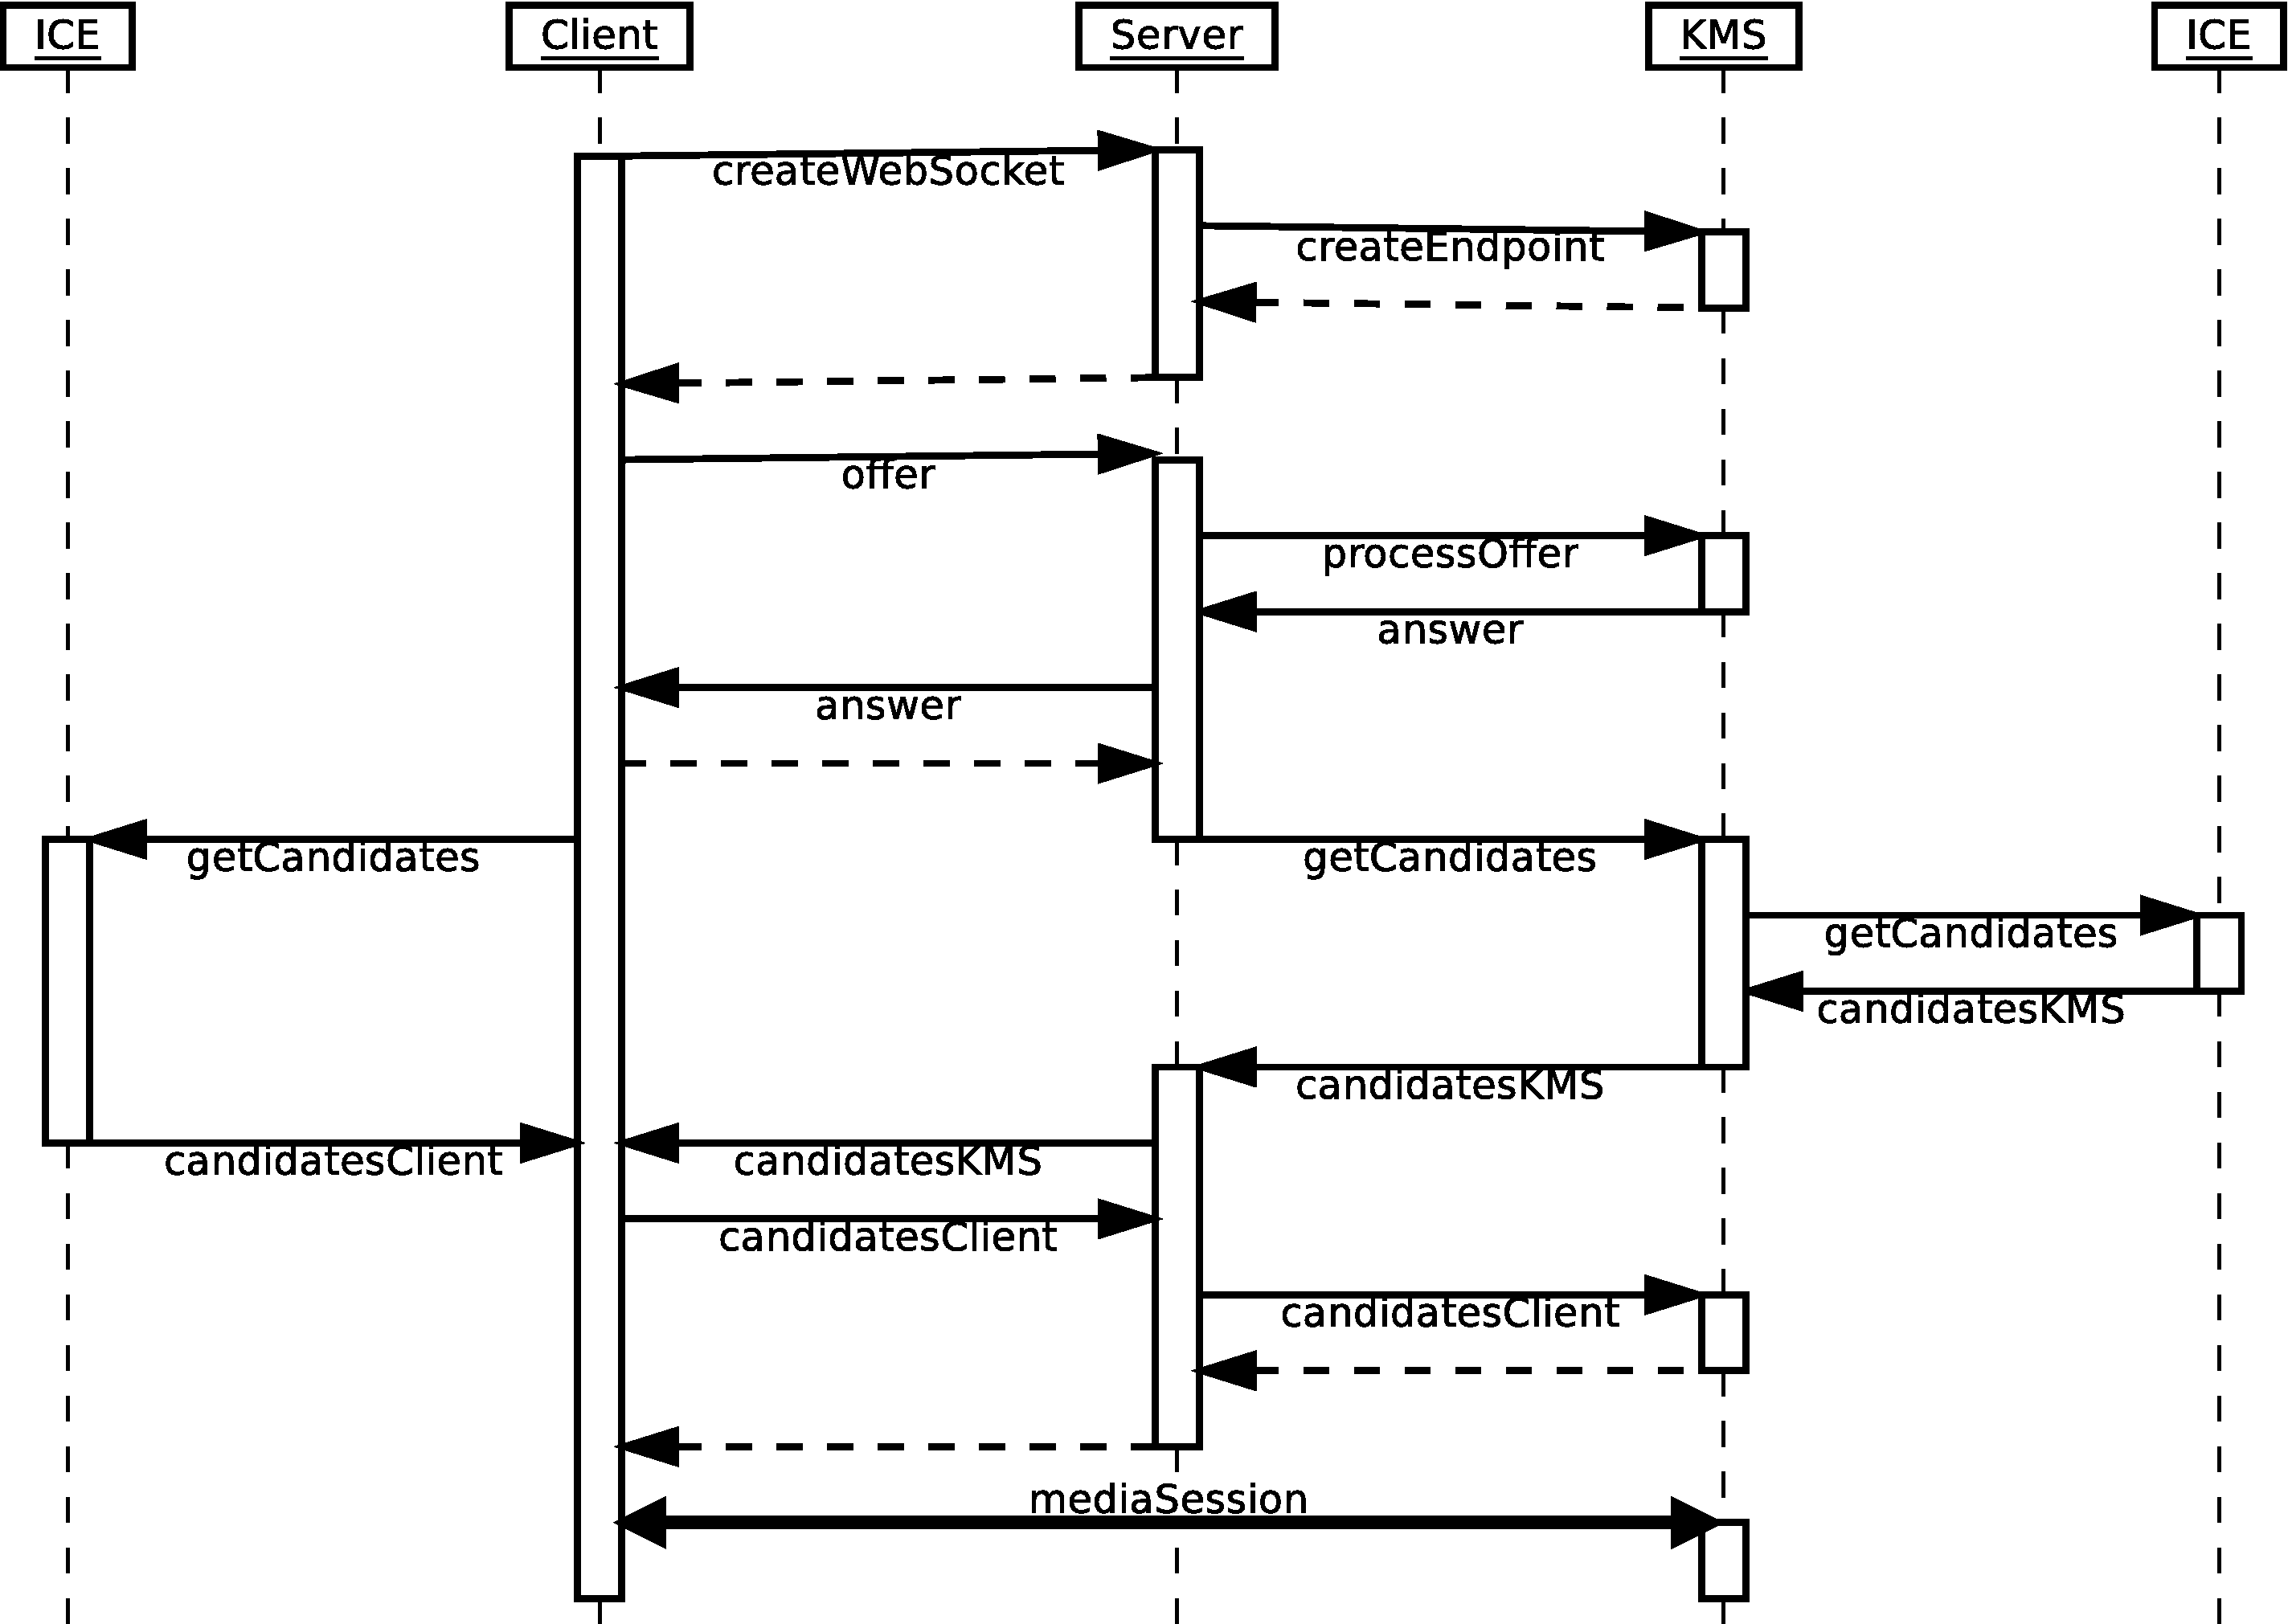
\includegraphics[width=\linewidth]{figures/signaling2}
    \caption{Signaling sequence diagram}
    \label{fig:signaling2}
\end{figure} 

Having the media session established, \gls{KMS} starts to record any received stream, combines all the streams into a single one (which is also recorded) and the client creates an \gls{URL} correspondent to the stream location.
Figure \ref{fig:devices} shows a combined stream with two different views of the same user with two cameras.
%One of our concerns was the storage scalability. 
%Saving files directly into the file system would require an extra effort to distribute and replicate files among servers.
\emph{Kurento Repository}\footnote{\url{http://doc-kurento-repository.readthedocs.org} (accessed on 17 March 2016)} provides a scalable, replicated storage solution for streams, based on \emph{MongoDB}.
Streams are saved into blocks of 10 seconds.

With server side recording, the user keeps the same stream \gls{URL} even if it is playing real time video or reproducing recorded video. 
It is \gls{KMS} that sends different content through that stream.
When a user desires to play recorded video, he uses the time bar, shown in Figure \ref{fig:timeline}, to select a bookmark or simply drags it backwards.
In response, the client uses the \emph{WebSocket} to send a message specifying the time and the intended user id.
The server performs the calculations in order to find a block that intersects the requested time, plays it and when finished, the next part is automatically played without the user intervention.

	\begin{figure}
		\centering
		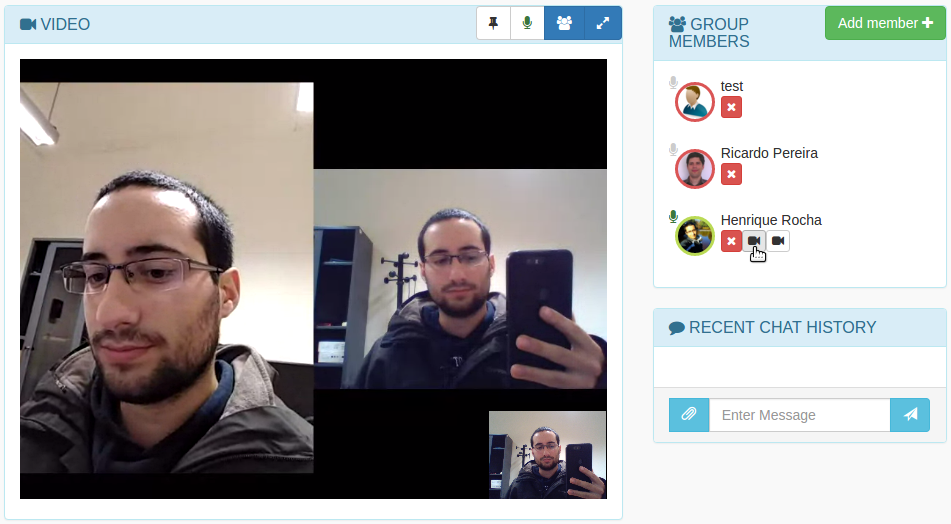
\includegraphics[width=\linewidth]{figures/devices.png}
		\caption{Multiple devices per user}
		\label{fig:devices}
	\end{figure}

	\begin{figure}
		\centering
		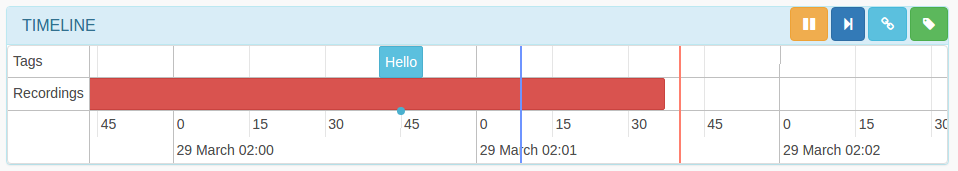
\includegraphics[width=\linewidth]{figures/timeline.png}
		\caption{Interactive timeline}
		\label{fig:timeline}
	\end{figure}




Our system supports creating content superimposed on the video.
This is achieved by creating \gls{HTML} tags on top of the video, with the same size.
The decision of which content to be displayed to each user is performed by our content scheduler, that uses the user's current time in order to synchronize which content is shown or removed from the user interface.

In order to create content, the user has the option to write simple movie captions without writing any code, otherwise, as mentioned before, it can write \gls{HTML}, \gls{CSS} and \emph{JavaScript}.

As manually content insertion is a laborious task that can be realized after the video is recorded, we provide an alternative mechanism for real time introduction of superimposed content.
In order to help the content creator to introduce and synchronize its content in real time, we allow the user to encode its content into \gls{QR} codes and show it to the camera in real time.
The \gls{QR} code processing is performed at \gls{KMS} and its content is returned by our content scheduler.


Our collaborative editor is a simple text editor, that is synchronized with all participants within a conference room, implemented using \emph{ot.js}.
The state of our collaborative editor is not saved on the database every time it changes.
Instead, the users just synchronize the editor content among themselves using the application server to relay editor changes and save on demand.



\section{Evaluation}
\label{chapter:evaluation}


We tested our solution with real users for a better understanding of their difficulties and what can be done in order to improve our solution's usability.
We have also tested the performance of our solution by measuring the used resources.
Those performance tests are crucial to ensure that our solution is in fact stable and scalable.

We evaluated our system by running all the backend components as Docker containers on a Debian 8 machine with 128GB of \emph{RAM}, 2 Intel Xeon E5-2640V2 CPUs, hybrid \emph{SSD}, \emph{HDD} storage and 1 Gbps Ethernet. 
We implemented a small \emph{Python} script using \emph{psutil}\footnote{\url{https://github.com/giampaolo/psutil} (Accessed March 27, 2016)} that collects, every second, CPU and physical memory information relative to each running process and network usage relative to each interface. 

The performance test scenario consists of having 7 users join the conference room sequentially and then leaving it, one at a time.
Each event, occurs with intervals of one minute, for a total of thirteen minutes (780 seconds).
  
From the media server perspective, if there are $n$ clients connected, each of them sending and receiving one stream, it is expected that server sends and receives also $n$ streams.
As such, we expect that the amount of network traffic increases linearly as users join a conference room.
Figure \ref{fig:test_full_features_net} confirms our expectations.
Each vertical yellow line represents one event: the first seven events are users entering the conference room, the next ones represent users leaving the conversation. 
     

\begin{figure}
  \centering
  %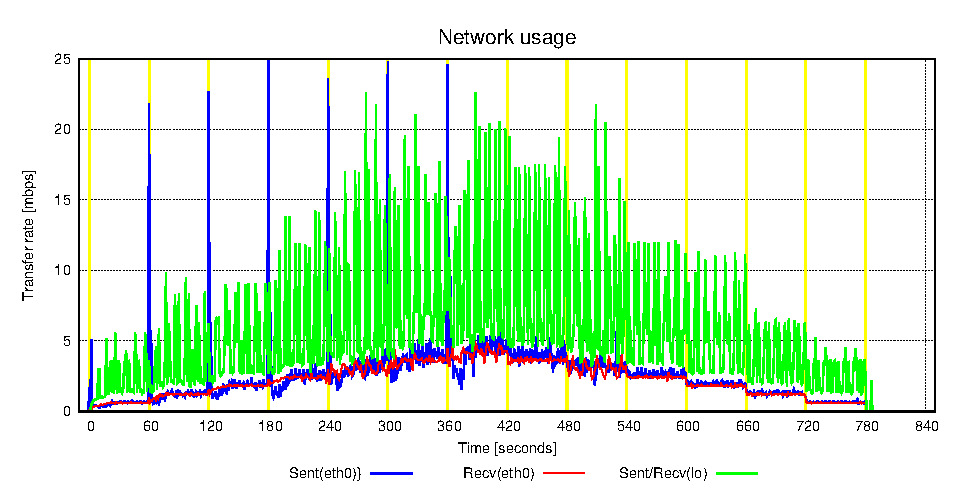
\includegraphics[width=\linewidth]{stats/test_full_features_net.eps}
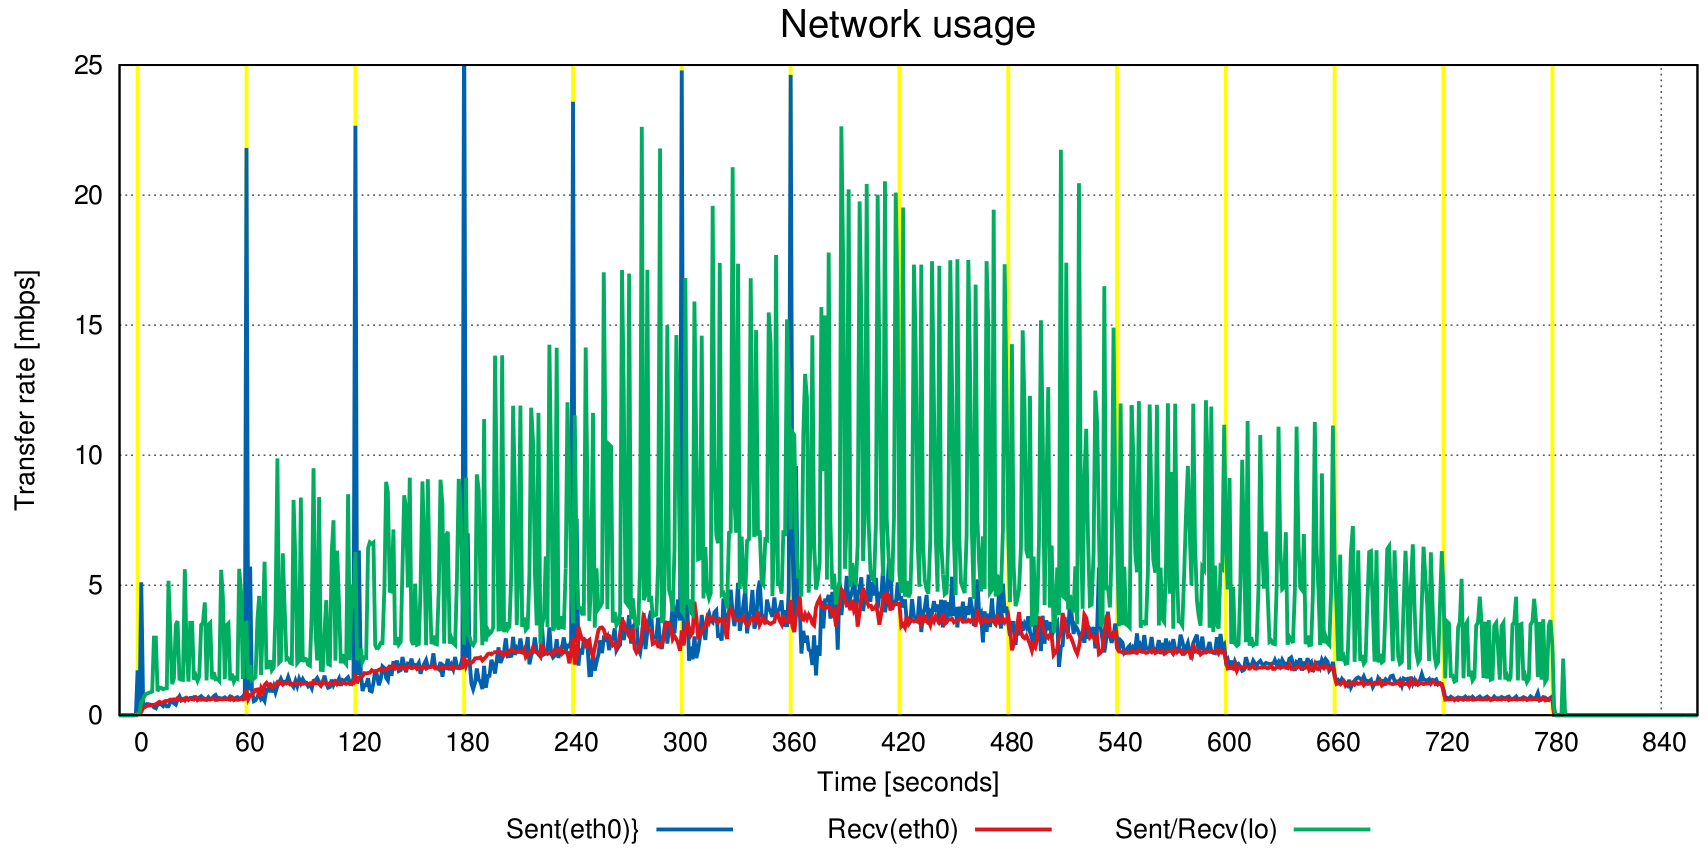
\includegraphics[width=\linewidth]{net_usage.png}
  \caption{Server network usage}
  \label{fig:test_full_features_net}
\end{figure}


The blue peaks are caused by the signaling phase and web page download when a new client joins.
The green peaks are inter-container traffic, caused by video and audio being transfered between \gls{KMS} and \emph{MongoDB} through \emph{Kurento Repository}.
Peaks occurs every 10 seconds, when a block of video is recorded.
The recordings are synchronized, so all user and mixed blocks start and end at the same time.
%That is why the amount of work done every ten seconds accumulates, and because this is performed locally, the maximum transfer rate is limited by the performance of the memory as buffers are written to buffers then to disks. 
Received data transfer rate has no significant peaks as \gls{HTTP} requests and signaling information contains little information, being mostly made up of video streams sent by the clients. % Esta frase estava um bocado sem sentido (olhando para a figura, no grafico mostra o ponto de vista do servidor, a frase estava no ponto de vista do utilizador)
As expected, sent and received traffic grows linearly with the number of users.

%candidato a apagar
%With this results we conclude that if we want to scale our storage solution using the \emph{MongoDB}'s cluster configuration, both \emph{Kurento Repository} and \gls{KMS} should be installed on the same machine because the loopback interface can handle bigger transfer rates than the remaining network interfaces. Installing the repository on the same machine as a database node does not ensure that recorded videos are stored in the same machine, for this reason we would prefer installing \gls{KMS} and \emph{Kurento Repository} on the same machine.


Figure \ref{fig:test_client_net} shows the same events regarding network usage from the perspective of the client.
We observe that in the first seconds the client adjusts the video quality it sends to \gls{KMS} and maintains that upload rate throughout.
Whenever a new client enters the conference, we observe that \gls{KMS} decreases the video quality in order to instantaneously integrate a new user into the conference room.
After a while, \gls{KMS} realizes that the network can handle the increase of clients and sends the video with a better quality to every participant.
When a user leaves the conference room \gls{KMS} has no need to decrease the participant's video quality as less network bandwidth will be used.
As expected, the maximum bandwidth used is constant and independent from the amount of participants.

\begin{figure}
  \centering
  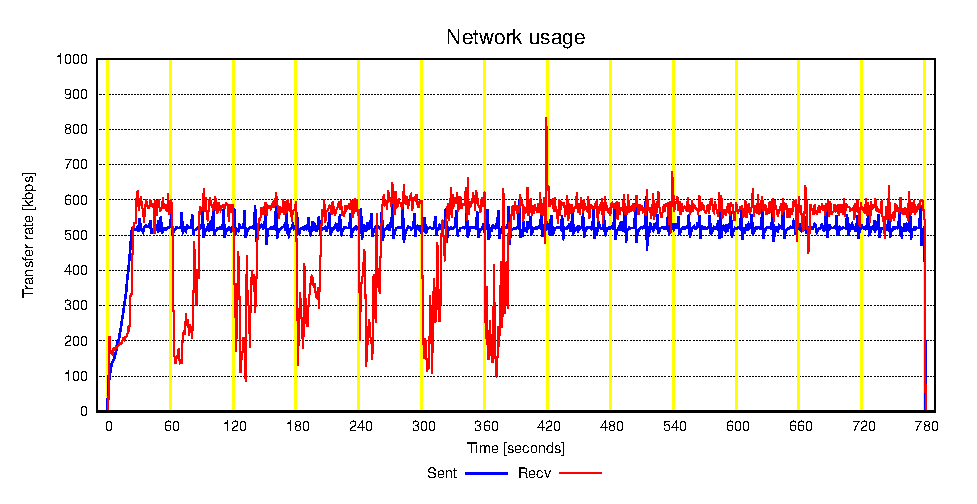
\includegraphics[width=\linewidth]{stats/test_client_net.eps}
  \caption{Client network usage}
  \label{fig:test_client_net}
\end{figure}

Figure \ref{fig:test_ram_fixed_mem} shows the memory usage during our performance test.
\gls{JVM}, \emph{MongoDB} and \gls{KMS} each perform their own memory management by holding and recycling objects when needed.
The expected and observed behavior of the memory usage is growth of memory usage while the users are entering the conference room and a memory usage stabilization afterwards.


\begin{figure}
  \centering
  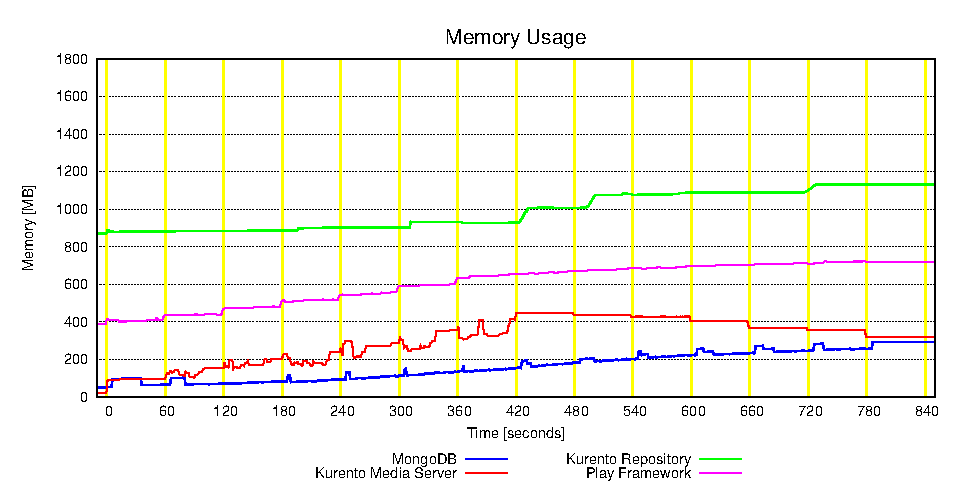
\includegraphics[width=\linewidth]{stats/test_ram_fixed_mem.eps}
  \caption{Server memory usage}
  \label{fig:test_ram_fixed_mem}
\end{figure}

\emph{MongoDB} memory usage keeps increasing because it tries to fit part of the database on \gls{RAM} for fast read access.
\emph{MongoDB} checkpoints data to disk every 60 seconds or when journal data exceeds 2GB\footnote{\url{https://docs.mongodb.org/manual/faq/storage/}(Accessed March 28, 2016)}, that explains the small memory usage peaks during our test case.
When the conference room is empty, there are no video recordings, which explains the memory stabilization at the end.
\emph{KMS} memory management released resources as soon as users left the room. 


Figure \ref{fig:test_full_features_cpu} shows the percentage of \gls{CPU} usage during our performance test case. 
Each 100\% represents one \gls{CPU} core, although that does not mean one \gls{CPU} is fully used, as e.g. two cores at 60\% represent 120\% \gls{CPU} usage.
As we can see, the percentage of \gls{CPU} used increases and decreases linearly in function of the number of conference participants.
As expected due to the video decoding and enconding and \gls{QR} code detection, \gls{KMS} is responsible for most of the \gls{CPU} usage.


\begin{figure}
  \centering
  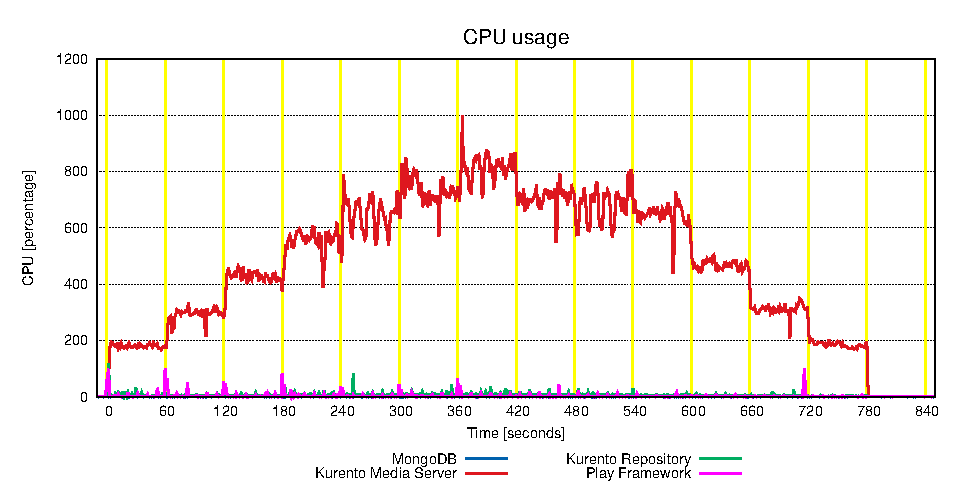
\includegraphics[width=\linewidth]{stats/test_full_features_cpu.eps}
  \caption{Percentage of CPU used during the performance tests}
  \label{fig:test_full_features_cpu}
\end{figure}

We conclude that our solution's bottleneck is the \gls{CPU} usage by \gls{KMS}.
We repeated the same test with \gls{QR} code detection disabled and verified that \gls{CPU} usage dropped to half.




In order to evaluate the usability of our solution, we performed usability tests with the help of 20 users with different backgrounds and ages between 22 and 38 years. 
Users were given a guide with five tasks to perform.
%The metrics we used were: number of clicks, number of errors and time spent. 
As a baseline, we used experienced users in order to retrieve the optimal task duration.


From the data collected with twenty tests with users, we have calculated the confidence intervals in order to understand the most plausible values for each metric.
As a result of both true average and variance being unknown and the usage of a relatively small amount of samples, we had to use the \emph{t-distribution} to estimate our metrics confidence intervals.
We have used a 95\% confidence level.

Task duration, shown in Figure \ref{fig:user_times}, as expected, was larger than that of an experienced user.
Curiously, there is no correlation between time taken by experienced and novice users.

\begin{figure}
  \centering
    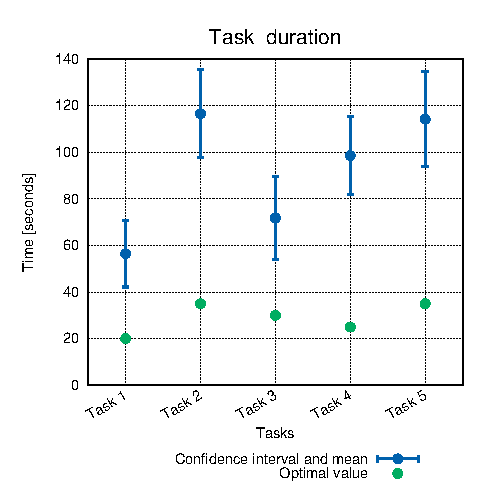
\includegraphics[width=0.75\linewidth]{stats/user_times.eps}
    \caption{Time spent per task}
    \label{fig:user_times}
\end{figure}

In Figure \ref{fig:user_diffs}, we can observe that most users had less difficulties with the task one (login in, accept and create friends) and two (create conference, share screen and use text editor), which represents types of tasks that most users are familiar with.
New concepts, such as navigate in time, manipulate annotations and create content (respectively \emph{task3}, \emph{task4} and \emph{task5}) turned out to be more difficult.
 Most of those difficulties, based on the users feedback, were mainly due to those concepts not being familiar to them.


\begin{figure}
  \centering
    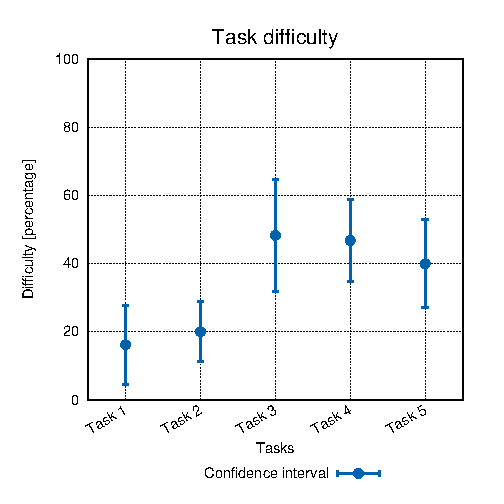
\includegraphics[width=0.75\linewidth]{stats/user_diffs.eps}
  \caption{Difficulty per task}
  \label{fig:user_diffs}
\end{figure}


As we had relatively bad results with some users, we explained to those users that could not conclude the tasks or performed them incorrectly, the most efficient way to perform the requested tasks.
Some users suggested to display more hints in order to achieve a faster learning.
Afterwards, all said they were impressed with the new functionality.

Most users gave us worse evaluations on our user interface layout and content editor, which was due to having a lot of tools present in the same web page and some of them being hidden due the screen size.
In some cases users had to scroll down in order to find the tools they were looking for. 

Another weak aspect was our content editor, which, in fact, we recognize is difficult to work with, mostly due to the amount of information that is necessary to create a synchronized content (starting time, duration and the content itself).
Some users have suggested that the content should also be present on the timeline so they could be easily dragged and resized (on time).

In conclusion, 100\% of our testers though that our solution was an innovation and 95\% recommended using our solution.




\section{Conclusions}
\label{chapter:conclusion}

We have successfully implemented a collaboration application that provides video-conferencing, chat, document editing and file sharing, with a novel concept: the ability to navigate back and forth in time, enabling non-linear visualization of video-conferencing.
This also makes it possible for users to enrich the video-content with hyper-media after it is created.

The performance tests that we have executed showed that our system is stable and more importantly, that our application server is lightweight and most of the processing power is dedicated to the streaming server.

Our usability tests showed that users had difficulty using this new concept, even though they found it useful and were willing to use it in the future.
This suggests that the user interface has to be improved, possibly by reducing some of the functionality in order to simplify it.

We are also aware of other limitation that would prevent our prototype from being deployed on a wide scale.
We have purposely chosen functionality over security when allowing users to provide code that is executed by other users.
A balance can be stroke by liming the flexibility afforded to users.

Our performance tests revealed that the streaming component uses a lot of resources, increasing the costs of a large deployment.
We left for a future work a deep analysis of the scalability of our system.

A useful feature when reviewing past video, is playback at a faster rate.
This is not possible using the current version of \gls{KMS}.
Even though we expect the availability of that feature in a near future, an alternative way to implement faster playback would be to use an external application, such as \emph{ffmpeg} to convert the video before playing it.

\section*{Acknowledgments}

This work was partially supported by national funds through Fundação para a Ciência e a Tecnologia (FCT) with reference UID/CEC/50021/2013.
This work has received funding from the European Union’s Horizon 2020 research and innovation program under grant agreement No 645342; project reTHINK.

% trigger a \newpage just before the given reference
% number - used to balance the columns on the last page
% adjust value as needed - may need to be readjusted if
% the document is modified later
%\IEEEtriggeratref{8}
% The "triggered" command can be changed if desired:
%\IEEEtriggercmd{\enlargethispage{-5in}}


\bibliographystyle{IEEEtran}
\bibliography{../tese2/references}


\end{document}


\grid
